\documentclass{kdp} % utf8,utf8x
%\usepackage[utf8]{inputenc}

\usepackage{mystyle} 
\usepackage{customcolors}
\usepackage{mycommands}

% Title
\title{A Book Template}
\author{\scalebox{0.91}{By: \link{https://github.com/alexanderthclark}{Alexander Clark}}}
\vspace{4cm}
\date{\scalebox{.8}{This version: \today}}

% name the list of listings 
\renewcommand\lstlistlistingname{Code} 
%\setcounter{tocdepth}{1}

\begin{document}

\frontmatter
\maketitle


\vfill 
% State your copyright details as desired. 
% You might instead use the doclicense package 
% https://ctan.org/pkg/doclicense?lang=en
% Then simply add \doclicenseThis

Copyright Informatation Here. 



%\doclicenseThis

\vspace{5cm}

%\vfill
%\thispagestyle{empty}

\tableofcontents
%% Add list of listings for code
\lstlistoflistings

\newpage

% I use * to make these unnumbered and then manually add to the toc

\chapter*{Preface}
\addcontentsline{toc}{chapter}{Preface}
\markboth{}{Preface}

\section*{Text Organization}
\addcontentsline{toc}{section}{Text Organization}
This text is not at all organized. 


\mainmatter

% Part I --------------------------------

\clearpage
\epigraphhead[200]{\vspace{4cm}\hfil\includegraphics[width = .8\textwidth]{moonbranch.jpg}\hfil\\
\begin{center}
\link{https://commons.wikimedia.org/wiki/File:Gold_Olive_Branch_Left_on_the_Moon_by_Neil_Armstrong_-_GPN-2002-000070.jpg}{Olive branch left on the Moon by Neil Armstrong.}\end{center}}

\part{First Part}\label{part:p1}

\chapter{First Chapter}\label{chapter:c1}
\chaptermark{$1^{\text{st}}$ Chapter} % change header

This is chapter one. 
\section{Fine}
This is a section.
\subsection{Finer}
This is a subsection. 


\chapter{Second Chapter}
This chapter follows Chapter \ref{chapter:c1}.

% Part II --------------------------------
\cleardoublepage
\epigraphhead[200]{\vspace{5cm}\hfil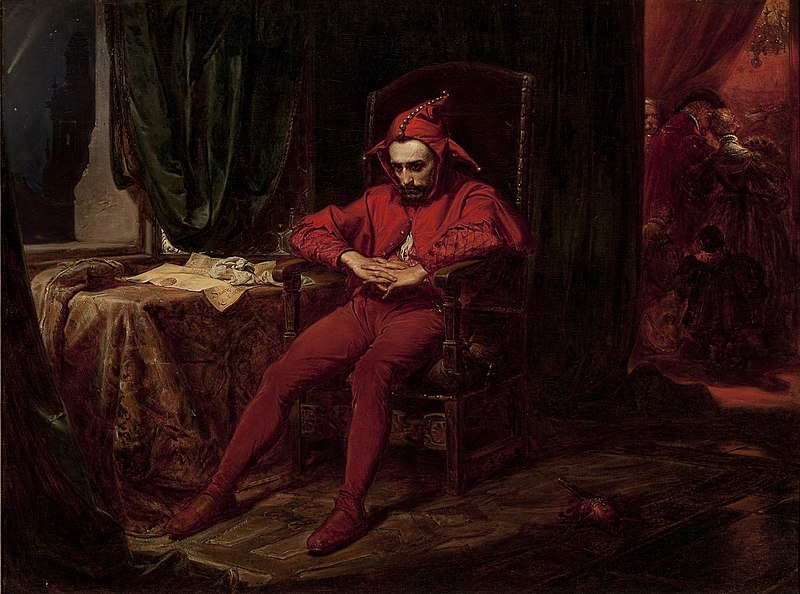
\includegraphics[width = .9\textwidth]{Stanczyk.jpg}\hfil\\
\begin{center}\link{https://en.wikipedia.org/wiki/Stańczyk_(painting)}{\emph{Stanczyk} by Jan Matejko} 
\end{center}}


\part{Last Part}\label{part:math}
This is the last part. It has no chapters. But here is a code block including an \code{if} statement.
\begin{lstlisting}[language = Python, caption = {[ifstatement.py]}]
x = 10
if x > 10:
    print('wow')
else:
    print('oh')
\end{lstlisting}

\nocite{stanczyk}
\nocite{10.3792/pia/1195572786} % get in some extra cites with \nocite

% Back Matter  --------------------------------
\backmatter

\printbibliography
%\printbibliography[heading=bibintoc, title = {References}]
%hey
%Filters bibliography
%\section*{References}
%\printbibliography[heading=subbibintoc, keyword={guides},title={Visualization Guides}]
%\printbibliography[heading=subbibintoc, keyword={nondata},title={Other}]


\chapter*{About the Author}
\faHandPeaceO
\end{document}




\end{document}